\documentclass[a4paper,12pt]{article}
\usepackage[top = 2.5cm, bottom = 2.5cm, left = 2.5cm, right = 2.5cm]{geometry}
\usepackage[T1]{fontenc}
\usepackage[utf8]{inputenc}
\usepackage{multirow} 
\usepackage{booktabs} 
\usepackage{graphicx}
\usepackage[spanish]{babel}
\usepackage{setspace}
\setlength{\parindent}{0in}
\usepackage{float}
\usepackage{fancyhdr}
\usepackage{amsmath}
\usepackage{amssymb}
\usepackage{amsthm}
\usepackage[numbers]{natbib}
\newcommand\Mycite[1]{%
	\citeauthor{#1}~[\citeyear{#1}]}
\usepackage{graphicx}
\usepackage{subcaption}
\usepackage{booktabs}
\usepackage{etoolbox}
\usepackage{minibox}
\usepackage{hyperref}
\usepackage{xcolor}
\usepackage[skins]{tcolorbox}
%---------------------------

\newtcolorbox{cajita}[1][]{
	 #1
}

\newenvironment{sol}
{\renewcommand\qedsymbol{$\square$}\begin{proof}[\textbf{Solución.}]}
	{\end{proof}}

\newenvironment{dem}
{\renewcommand\qedsymbol{$\blacksquare$}\begin{proof}[\textbf{Demostración.}]}
	{\end{proof}}

\newtheorem{problema}{Problema}
\newtheorem{definicion}{Definición}
\newtheorem{ejemplo}{Ejemplo}
\newtheorem{teorema}{Teorema}
\newtheorem{corolario}{Corolario}[teorema]
\newtheorem{lema}[teorema]{Lema}
\newtheorem{prop}{Proposición}
\newtheorem*{nota}{\textbf{NOTA}}
\renewcommand\qedsymbol{$\blacksquare$}
\usepackage{svg}
\usepackage{pgfplots}
\pgfplotsset{compat=1.11}

\usepackage{tikz}
\usetikzlibrary{calc}

\usetikzlibrary{patterns}
\usepackage[framemethod=default]{mdframed}
\global\mdfdefinestyle{exampledefault}{%
linecolor=lightgray,linewidth=1pt,%
leftmargin=1cm,rightmargin=1cm,
}




\newenvironment{noter}[1]{%
\mdfsetup{%
frametitle={\tikz\node[fill=white,rectangle,inner sep=0pt,outer sep=0pt]{#1};},
frametitleaboveskip=-0.5\ht\strutbox,
frametitlealignment=\raggedright
}%
\begin{mdframed}[style=exampledefault]
}{\end{mdframed}}
\newcommand{\linea}{\noindent\rule{\textwidth}{3pt}}
\newcommand{\linita}{\noindent\rule{\textwidth}{1pt}}

\AtBeginEnvironment{align}{\setcounter{equation}{0}}
\pagestyle{fancy}

\fancyhf{}









%----------------------------------------------------------
\lhead{\footnotesize Geometría diferencial}
\rhead{\footnotesize  Rudik Roberto Rompich}
\cfoot{\footnotesize \thepage}


%--------------------------

\begin{document}
 \thispagestyle{empty} 
    \begin{tabular}{p{15.5cm}}
    \begin{tabbing}
    \textbf{Universidad del Valle de Guatemala} \\
    Departamento de Matemática\\
    Licenciatura en Matemática Aplicada\\\\
   \textbf{Estudiante:} Rudik Roberto Rompich\\
   \textbf{Correo:}  \href{mailto:rom19857@uvg.edu.gt}{rom19857@uvg.edu.gt}\\
   \textbf{Carné:} 19857
    \end{tabbing}
    \begin{center}
        Geometría diferencial - Catedrático: Alan Reyes\\
        \today
    \end{center}\\
    \hline
    \\
    \end{tabular} 
    \vspace*{0.3cm} 
    \begin{center} 
    {\Large \bf  Tarea
} 
        \vspace{2mm}
    \end{center}
    \vspace{0.4cm}
%--------------------------
\section{Problema}
\begin{problema}[Problema D]
    Resolver:  
    \begin{itemize}
        \item  Defina los términos “opción”, “call” y “put”. Asimismo, explique cuál es la diferencia principal entre las opciones europeas y americanas.
        \begin{sol}
            A continuación se listan las definiciones: 
            \begin{itemize}
                \item  Una opción hace referencia a un contrato que da a su comprador el derecho (pero no la obligación) a comprar o vender activos subyacentes (es decir, acciones, índices bursátiles, etcétera) a un precio de ejercio $(K)$ hasta una fecha límite ($T$). Las opciones se dividen en dos clases: las \textit{call} (las de compra) y las \textit{put} (las de venta).
                \item Una opción \text{call} es una opción de compra. En este caso, otorga a su titular el derecho de comprar un activo subyacente a un precio de ejercicio ($K$) en o antes de una fecha de vencimiento ($T$). El titular de la opción de compra se beneficiaría si el precio del activo subyacente ($S_t$) en la fecha de vencimiento es mayor que el precio de ejercicio ($S_T > K$). En este caso, el beneficio sería la diferencia entre el precio del activo subyacente y el precio de ejercicio ($S_T - K$).
                \item 
                Algunos aspectos interesantes: 
                \begin{itemize}
                    \item Todas las subidas en bolsa por encima del precio fijo, serán ganancias. Si cae por debajo, las pérdidas son siempre fijas y conocidas con antelación, iguales a la cantidad que se pago por la opción \textit{call} (prima).
                    \item La función de pago (payoff) de una opción de compra se puede describir como:
                        $$\text{Payoff}_\text{call}(S_T, K )=\max(S_ 
                        T-K,0)$$
                    \item El valor de una opción \textit{call} se calcula utilizando el Modelo de Black-Scholes (la ecuación diferencial general): 
                    $$\frac{\partial f}{\partial t}+rS \frac{\partial f}{\partial S}+\frac{1}{2}\sigma^2 S^2 \frac{\partial ^2 f}{\partial S^2}=rf$$
                    con la condición de frontera en $t=T$, 
                    $$f=\text{Payoff}_\text{call}(S_T, K )=\max(S_T-K,0)$$
                    
                    y dando como resultado
                    $$C(S_0,T) = S_0N(d_1) - Ke^{-rT}N(d_2)$$
                \end{itemize}
                 

                \item Una opción \textit{put} es una opción de venta. Otorga al comprador el derecho de vender un activo subyacente a un precio de ejercicio ($K$) en o antes de una fecha de vencimiento ($T$). El comprador de la opción de venta se beneficiaría si el precio del activo subyacente ($S_t$) en la fecha de vencimiento es menor que el precio de ejercicio ($S_T < K$). En este caso, el beneficio sería la diferencia entre el precio de ejercicio y el precio del activo subyacente ($K - S_T$). Algunos aspectos interesantes: 
                \begin{itemize}
                    \item El dueño o comprador de una opción \textit{put} se beneficia de la opción si el activo subyacente baja.
                    \item La función de pago (payoff) de una opción de venta se describe como:

                    $$\text{Payoff}_{put}(S_T,K)=\max(K-S_T,0)$$
                    \item El valor de una opción Put se calcula utilizando el Modelo de Black-Scholes (la ecuación diferencial general): 
                    $$\frac{\partial f}{\partial t}+rS \frac{\partial f}{\partial S}+\frac{1}{2}\sigma^2 S^2 \frac{\partial ^2 f}{\partial S^2}=rf$$
                    con la condición de frontera en $t=T$, 
                    $$f=\text{Payoff}_{put}(S_T,K)=\max(K-S_T,0)$$
                    y dando como resultado:
                    $$P(S_0,T) = Ke^{-rT}N(-d_2) - S_0N(-d_1)$$
                \end{itemize}
                
            \end{itemize}
    
        
 Donde:
 \begin{itemize}
    \item $C(S_0,T)$ es el valor de una opción \textit{call}
    \item $P(S_0,T)$ es el valor de una opción \textit{put}
    \item $T$ es el tiempo restante de la opción con plazo total en ese momento
    \item $r$ es la tasa de interés congruente con el plazo restante de la opción
    \item $K$ es el precio base (conocido como \textit{Strike price}), definido como parte del contrato
    \item $S_0$ es el precio actual del activo subyacente
    \item $N(x)$ es la función de distribución normal acumulada
    \item $d_1$ y $d_2$ se calculan como: $$d_1 = \frac{\ln(S_0/K) + (r + \sigma^2/2)T}{\sigma \sqrt{(T-t)}}$$
     $$d_2 = d_1 - \sigma \sqrt{T}$$ donde $\sigma$ es la volatilidad futura del activo subyacente.
    
 \end{itemize}

 Ahora bien, ¿cuál es la diferencia principal entre las opciones europeas y americanas? Básicamente la diferencia es el momento en que el dueño de la opción ejerce el contrato.
 \begin{itemize}
    \item \textbf{Americanas}:  Estas opciones pueden ejercerse en cualquier momento desde la fecha de emisión hasta la fecha de vencimiento ($t \in [0, T]$). Por lo tanto, el titular de una opción americana tiene más versatilidad que el titular de una opción europea, ya que puede decidir cuándo ejercer la opción considerando cualquier condición del mercado y sus expectativas.
    \item \textbf{Europeas}: Estas opciones solo pueden ejercerse en la fecha de vencimiento ($T$). En otras términos, el titular de una opción europea tiene el derecho de comprar (en el caso de una opción de compra o call) o vender (en el caso de una opción de venta o put) el activo subyacente únicamente en la fecha límite de vencimiento especificada en el contrato de la opción.
 \end{itemize}

 Por ejemplo, supóngase el siguiente caso:
 \begin{itemize}
    \item Americana 
    \begin{itemize}
        \item Se compra una opción americana a un precio de ejercicio de \$100.
        \item El precio de la acción sube a \$120 antes de la fecha de vencimiento de la opción. 
        \item Se ejerce el derecho a comprar las acciones a \$100 y luego venderlas a \$120.
        \item Se obtiene \$20 de ganacia por acción.
    \end{itemize}
    \item Europea
    \begin{itemize}
        \item Se compra una opción europea a un precio de ejercicio de \$100.
        \item El precio de la acción sube a \$120 antes de la fecha de vencimiento de la opción. 
        \item No se puede ejercer el derecho a comprar las acciones a \$100 y luego venderlas a \$120. Ya que aún no ha llegado la fecha límite. 
        \item Llegando a la fecha límite la opción baja a \$90. 
        \item No se puede comprar la acción a \$100, sino que a \$90 y entonces no habría ganancia. 
    \end{itemize}
\end{itemize}

    
        \end{sol}
        
        \item Grafique el retorno al vencimiento de una exposición larga a una opción put europea.
        Señale claramente en el gráfico el precio de ejercicio y el valor correspondiente a la prima de la opción.
        \begin{sol}
            Para este problema, se consideraron los siguientes parámetros: 
            \begin{itemize}
                \item Precio de ejercicio $(K)$: \$50
                \item Prima de la opción: \$4 
            \end{itemize}
            Entonces, para graficar el retorno al vencimiento de una exposición larga a una opción put europea, se usó \textit{Mathematica}. De donde se generó el siguiente gráfico: 
            \begin{figure}[H]
                \centering
                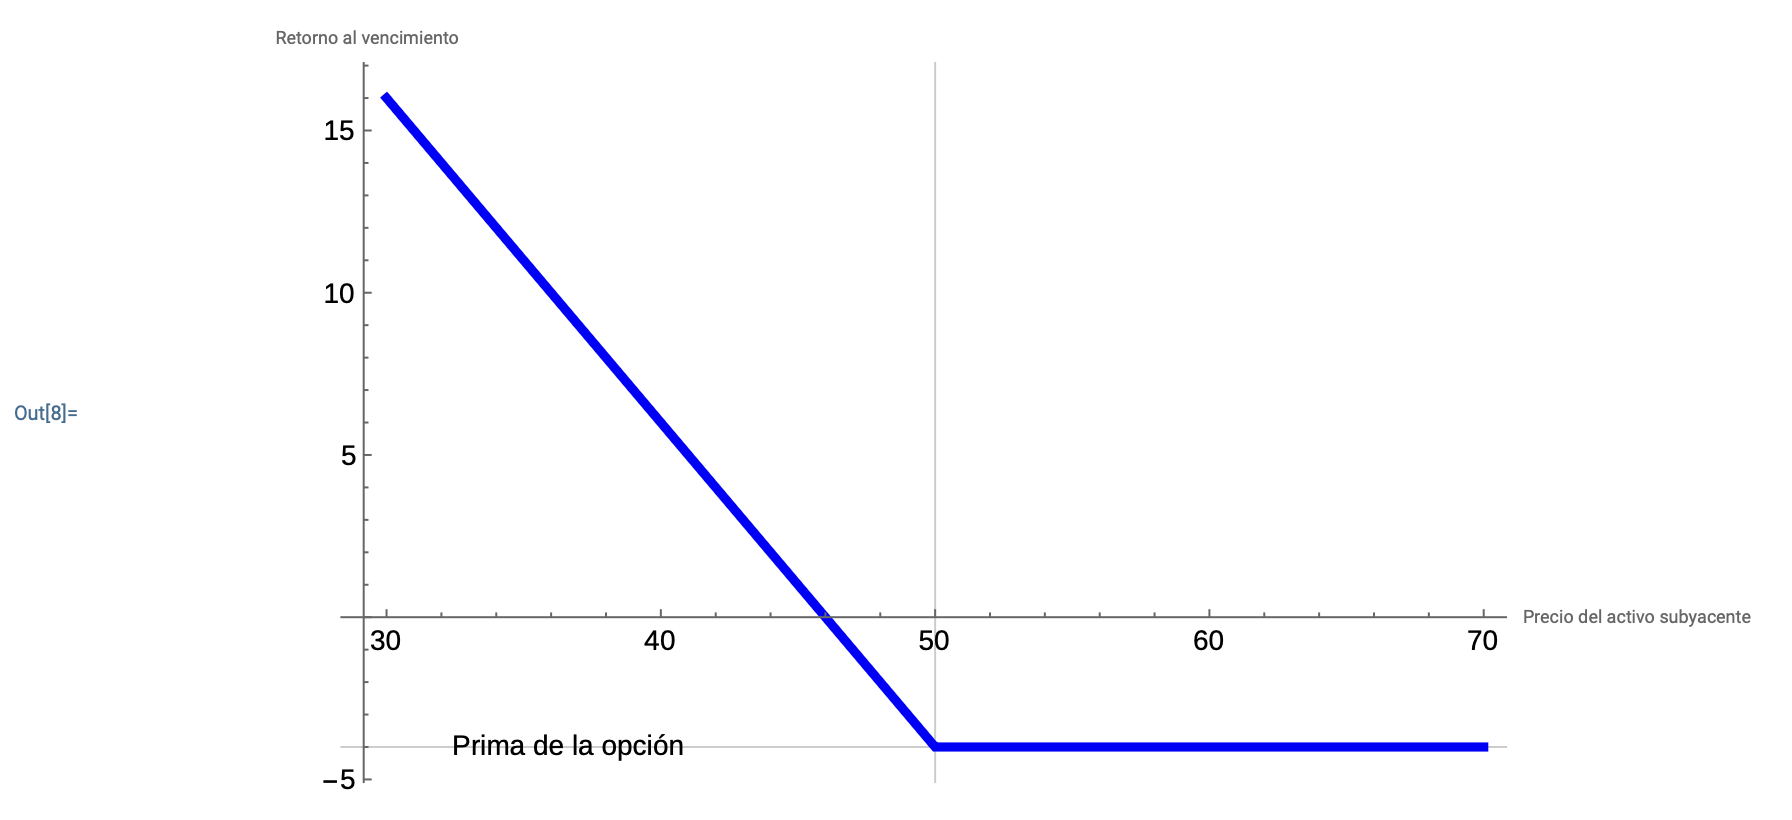
\includegraphics[scale=0.5]{imagenes/1.png}
            \end{figure}
            De esta gráfica generamos el siguiente análisis: 
            \begin{itemize}
                \item \textbf{Ejes}: El eje $x$ representa el precio del activo subyacente al vencimiento ($S_T$), mientras que el eje $y$ representa el retorno al vencimiento de la opción \textit{put}. El rango del eje $x$ se define entre un precio mínimo y un precio máximo para ilustrar cómo el retorno al vencimiento varía en función del precio del activo subyacente.
                \item \textbf{Línea azul}: Esta línea representa la función de retorno al vencimiento de una exposición larga a una opción \textit{put} europea. La función se calcula utilizando la siguiente fórmula:
                $$\text{Retorno al vencimiento}=\max(K-S_T,0)-\text{Prima}$$
                Donde $K$ es el precio de ejercicio, $S_T$ es el precio del activo subyacente al vencimiento.
                \item \textbf{Línea vertical gris}: Esta línea representa el precio de ejercicio ($K$) de la opción put. Señala el punto de quiebre a partir del cual el comprador de la opción put comenzaría a obtener beneficios si decide ejercerla al vencimiento. Cuando $S_T < K$, el comprador de la opción put obtiene beneficios al ejercer la opción, ya que puede vender el activo subyacente a un precio mayor ($K$) que su valor de mercado ($S_T$).
                \item \textbf{Línea horizontal gris}: Esta línea indica el valor correspondiente a la prima de la opción. La prima es el costo inicial que el comprador paga al adquirir la opción put. Esta línea muestra cómo el retorno al vencimiento de la opción put se ve afectado por la prima pagada. Aquí tenemos unos aspectos interesantes: 
                \begin{itemize}
                    \item Cuando el retorno al vencimiento es igual a la prima de la opción (con signo negativo), el inversor no obtiene beneficios ni pérdidas al ejercer la opción.
                    \item Si el retorno al vencimiento es mayor que la prima (con signo negativo), el inversor obtiene beneficios; de lo contrario, el inversor incurre en pérdidas.
                \end{itemize}
                
    

            \end{itemize}
           
        \end{sol}
        \item Brinde la interpretación más completa que le sea posible del precio teórico de un put,
        representado convencionalmente por la ecuación:
        $$p=Ke^{-rT}N(-d_2)-S_0 N(-d_1)$$
            No olvide aludir al marco teórico asociado con BSM. En su respuesta, aplique el concepto
        del “web of belief”, tomando como nodos centrales: la noción clásica del tiempo, la
        ausencia de interactividad entre sujeto y objeto, la unidad entre los espacios de estado y de
        observación, y la asociación que se hace entre eventos extremos e infrecuentes.

        \begin{sol}
            La ecuación en cuestión es la fórmula de Black-Scholes-Merton (BSM) para el precio teórico de una opción put europea. Cada uno de sus elementos en la ecuación ya se definieron en el primer subproblema. En primer lugar, comenzamos haciendo un análisis matemático de $p$, el cual se desprende de la ecuación diferencial de BSM:
            \begin{equation*}
                \frac{\partial f}{\partial t} + \frac{1}{2}\sigma^2 S^2 \frac{\partial^2 f}{\partial S^2} + rS\frac{\partial f}{\partial S} - rf = 0
                \end{equation*}
                Donde:
                \begin{itemize}
                    \item $f(S, t)$ es el precio de la opción como función del precio del activo subyacente $S$ y el tiempo $t$.
                    \item $\sigma$ es la volatilidad del activo subyacente.
                    \item $r$ es la tasa de interés libre de riesgo.        
                \end{itemize}

                Ahora bien, no resolveremos la ecuación diferencial rigurosamente. Pero se plantea un procedimiento general de los procemientos necesarios para resolverla. 
                \begin{enumerate}
                    \item Se considera un cambio de variable $x = \ln{S}$ y $\tau = T - t$, donde $T$ es el tiempo de vencimiento de la opción. La ecuación diferencial parcial se convierte en:
                    \begin{equation*}
                    \frac{\partial f}{\partial \tau} = \frac{1}{2}\sigma^2 \frac{\partial^2 f}{\partial x^2} + (r - \frac{1}{2}\sigma^2)\frac{\partial f}{\partial x} - rf
                    \end{equation*}
                    \item Se puede aplicar una transformación de Feynman-Kac, que relaciona la ecuación diferencial parcial con la expectativa condicional de un proceso estocástico. Esto lleva a:
                    \begin{equation*}
                    f(x, \tau) = e^{-r\tau} \mathbb{E} \left[ z(X_{\tau}) \middle| X_0 = x \right]
                    \end{equation*}
                    \item Se transforma la solución de vuelta a las variables originales $S$ y $t$.
                    \item Y como se mencionó en la clase, ya se puede aplicar la condición de frontera $f(S_T) = \max(K - S_T, 0)$. 
                    \item Con esto, generamos la ecuación de $p$.
                \end{enumerate}
                

Por otra parte, esta ecuación se basa en varios supuestos y conceptos fundamentales, que se analizan a continuación en el contexto del «web of belief» y los nodos centrales mencionados. Para ilustrarlo de una forma mejor, considérese el siguiente ejemplo, el cual se irá detallando en cada uno de los aspectos: 

\begin{cajita}
    Considérese una opción put europea en una acción ficticia: 
    \begin{itemize}
        \item Precio de ejercicio ($K$): 100 €
        \item Tasa de interés libre de riesgo ($r$): 2\% anual
        \item Tiempo hasta el vencimiento ($T$): 6 meses (0.5 años)
        \item Precio actual del activo subyacente ($S_0$): 95€
    \end{itemize}

    Su gráfica se vería de la siguiente manera: 

    \begin{figure}[H]
        \centering
        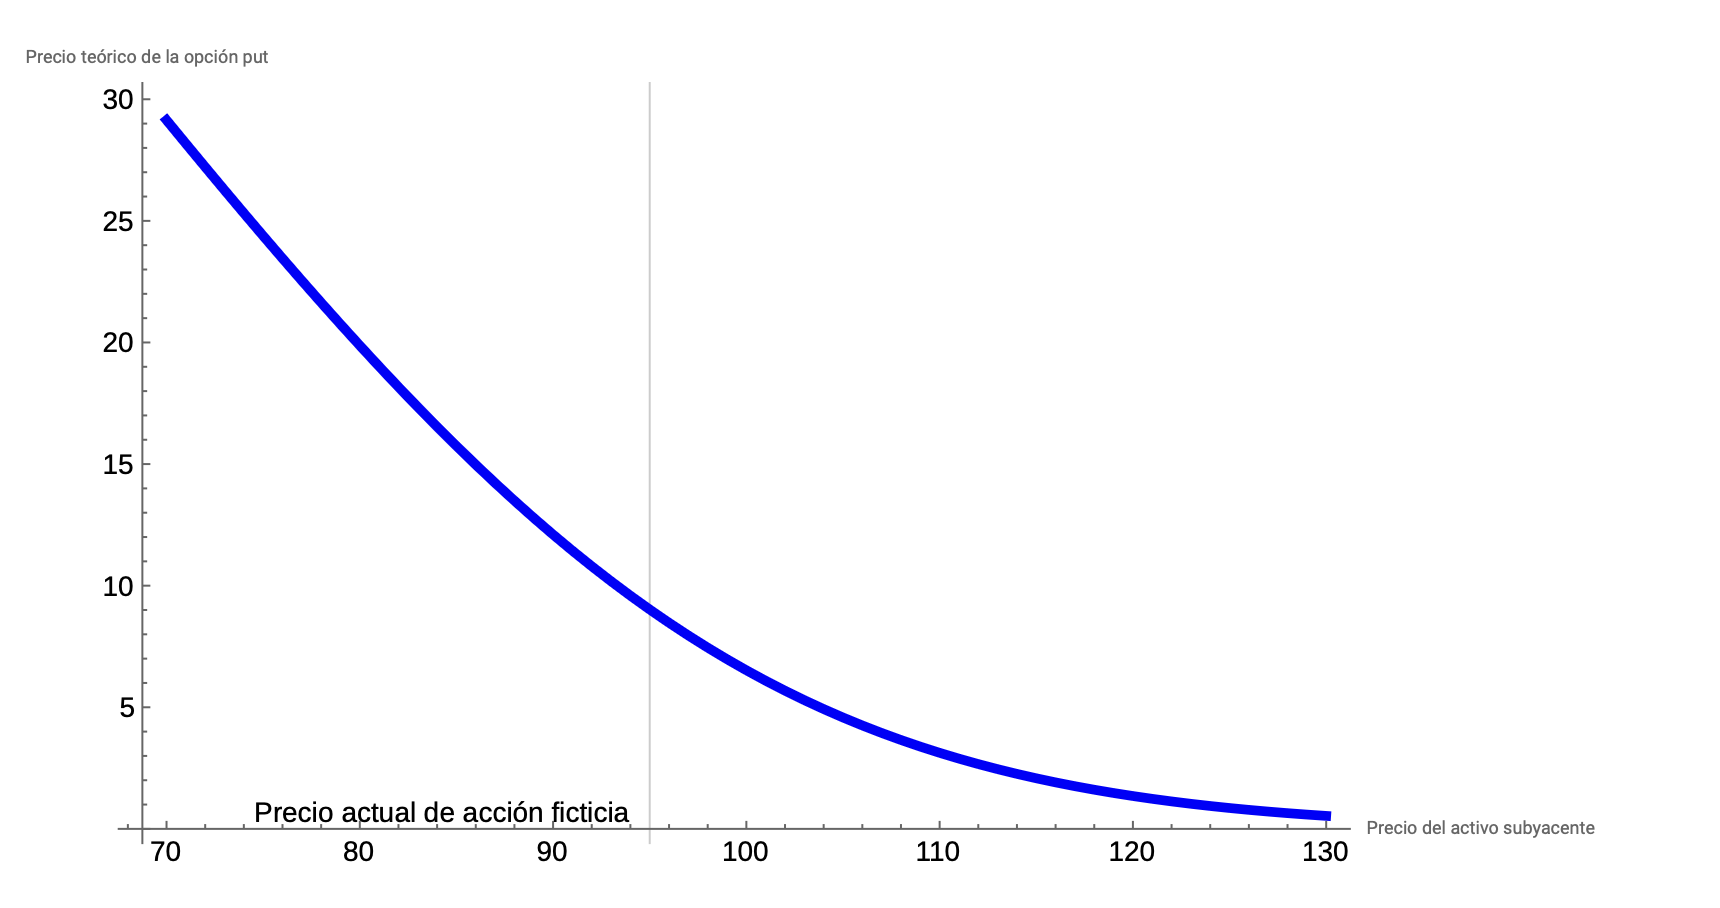
\includegraphics[scale=0.4]{imagenes/2.png}
    \end{figure}

\end{cajita}

\begin{itemize}
    \item \textbf{Noción clásica del tiempo}:  Primero, consideramos que el modelo de BSM toma como supuesto y considera que el tiempo avanza de manera continua y determinista (es decir que desde el principio se sabe lo que sucederá). Algunos aspectos importantes: 
    \begin{itemize}
        \item  En la ecuación diferencial de Black-Scholes utiliza una variable de tiempo $T$ que representa el vencimiento de la opción. 
    
       \item El factor de descuento $e^{-rT}$ en la ecuación considera la tasa de interés libre de riesgo ($r$) y el tiempo hasta el vencimiento ($T$), asumiendo que la tasa de interés se mantiene constante durante ese período.
        
        \item La noción clásica del tiempo es elemental para el modelo, ya que la evolución del precio del activo subyacente y la valuación de la opción dependen de la progresión del tiempo hacia el vencimiento.
    
    \end{itemize}
    \begin{cajita}
        En el \textbf{ejemplo} propuesto, la interpretación de la noción clásica sería que el tiempo hasta el vencimiento es de 6 meses (0.5 años). No importa si los inversores compran o venden la opción, el tiempo hasta el vencimiento no se ve afectado por sus acciones y sigue siendo constante. 
    \end{cajita}

    \item \textbf{Ausencia de interactividad entre sujeto y objeto}: En este sentido: 
    \begin{itemize}
        \item El modelo BSM asume que los inversores son tomadores de precios y no pueden influir en el precio del activo subyacente.
        \item Se asume que no hay costos de transacción o restricciones de venta en corto. Ya que en la vida real, sí existen esos factores, el cual no toma en cuenta BSM 
        \item En BSM, los inversores son los observadores pasivos del mercado y no tiene en cuenta la interacción entre los sujetos (inversores) y el objeto (activos financieros).
    \end{itemize}
    \begin{cajita}
        En el \textbf{ejemplo}, el precio de las acciones ficticias es de 95€. En este nodo, este precio no se verá influenciado por la compra o venta de opciones put en la acción ficticia.  Es decir, las acciones de los inversores en el mercado de opciones no afectarán el precio de las acciones de ninguna manera. 
    \end{cajita}
    
    \item \textbf{Unidad entre los espacios de estado y de observación}: Considerando esto, tenemos: 
    \begin{itemize}
        \item La ecuación BSM asume que el espacio de estado, es decir, el conjunto de todas las posibles realizaciones del precio del activo subyacente, es observable directamente.
        \item Esto implica que los inversores pueden observar y medir el precio del activo subyacente y su volatilidad en cualquier momento.
        \item En este contexto, no hay incertidumbre adicional o factores no observables que afecten el precio de la opción, lo que simplifica el proceso de valuación y hace que el modelo sea más fácil de aplicar en la práctica.
    \end{itemize}
    \begin{cajita}
        En el \textbf{ejemplo}, suponemos que conocemos el precio de las acciones  (95€), la tasa de interés libre de riesgo (2\% anual) y el tiempo hasta el vencimiento (6 meses); las cuales no tienen ninguna incertidumbre (según BSM), ya que en la vida real, naturalmente, esos valores podrían estar expuestos a la incertidumbre. 
    \end{cajita}
    
    
    \item \textbf{Eventos extremos e infrecuentes}: Considerando: 
    \begin{itemize}
        \item El modelo BSM supone que el precio del activo subyacente sigue un movimiento browniano geométrico con una volatilidad constante.
        \item La distribución de los rendimientos del activo subyacente es normal y, por lo tanto, los eventos extremos e infrecuentes no se tienen en cuenta adecuadamente en la valuación de la opción (es decir, no hay punto atípicos).
        
        \item En la vida real, los mercados financieros suelen experimentar eventos extremos (como crisis financieras, inflación, inyección de dinero por parte de la FED, tweets de Elon Musk, FOMO...) que pueden tener un impacto significativo en el precio de las opciones. La incapacidad del modelo BSM para abordar adecuadamente estos eventos extremos e infrecuentes es una de sus limitaciones.
    \end{itemize}
    \begin{cajita}
        En el \textbf{ejemplo}, esto significa que grandes cambios en el precio de las acciones ficticias son poco probables en un corto período de tiempo. Digamos, como suposición  que el precio de las acciones aumenta bruscamente a 1000€ (tipo \textit{Dogecoin} cuando Elon Musk sube un tweet) en un día debido a una noticia inesperada. El modelo BSM no captura adecuadamente este tipo de eventos extremos, ya que asume que los cambios en el precio siguen una distribución normal y por lo tanto, no anticipa estos movimientos extremos en el precio.
    \end{cajita}
    
\end{itemize}





        \end{sol}
        \item Si el mecanismo generador de precios del activo subyacente habita un espacio diferente al
        espacio de observación / medición, considere las circunstancias en las que BSM sigue siendo una representación útil del precio del put. En su respuesta aluda a los modelos
        caóticos, fractales y cuánticos, como alternativas al enfoque teórico clásico
        \begin{sol}

            Esta pregunta es compleja porque haría falta considerar modelos concretos en específico, los cuales se han mencionado en la clase, pero de igual forma, no se han estudiado a profundidad para dar una respuesta certera a esta pregunta. Sin embargo, algunos de los aspectos que tomaría en cuesta serían los siguientes: 
            \begin{itemize}
                \item  Aproximación en pequeñas secciones: A pesar de que los modelos caóticos, fractales y cuánticos pueden ofrecer una descripción más precisa de la dinámica del mercado, BSM puede proporcionar una aproximación razonable si se trata en «pequeñas secciones», imitando los parámetros necesarios de BSM 
                \item Calibración de modelos: BSM puede usarse como un punto de referencia para calibrar modelos más complejos y realistas. Los parámetros de modelos caóticos, fractales o cuánticos pueden ajustarse de tal manera que sus resultados se ajusten a los de BSM en ciertas condiciones del mercado. Luego, estos modelos más avanzados pueden usarse para analizar y predecir el comportamiento de los precios del activo subyacente en situaciones más extremas o complicadas.
                \item Cuando existe baja volatilidad: BSM puede ser útil en entornos de baja volatilidad, donde los cambios en el precio del activo subyacente son relativamente pequeños y siguen una distribución aproximadamente normal. En estas circunstancias, la suposición de BSM de que los precios siguen un movimiento browniano geométrico puede ser una aproximación aceptable, y los modelos caóticos, fractales o cuánticos podrían no ofrecer ventajas significativas.
                \item Opciones de corto plazo: Para opciones con vencimientos cortos, las diferencias entre BSM y modelos más avanzados pueden ser menos pronunciadas, ya que los efectos de eventos extremos y las características no lineales de estos modelos son menos relevantes en escalas de tiempo cortas. En tales casos, BSM puede proporcionar una estimación útil del precio del put.
            \end{itemize}



        \end{sol}
    \end{itemize}
   


\end{problema}


\section{Apéndices}

\begin{itemize}
    \item Código para generar el retorno al vencimiento de una exposición larga a una opción put europea.
    
\begin{verbatim}
    (* Parámetros *)
    strikePrice = 50; (* Precio de ejercicio (K) *)
    optionPremium = 4; (* Prima de la opción *)
    minPrice = 30; (* Precio mínimo del activo subyacente en el gráfico *)
    maxPrice = 70; (* Precio máximo del activo subyacente en el gráfico *)
    
    
    (* Función de retorno al vencimiento *)
    payoffPut[stockPrice_, strikePrice_, premium_] := 
    Max[strikePrice - stockPrice, 0] - premium;
    returnAtMaturity = Table[{price, payoffPut[price, strikePrice,
     optionPremium]},{price, minPrice, maxPrice}];
    
    (* Gráfico *)
    graph = ListLinePlot[returnAtMaturity, 
      PlotRange -> All,
      AxesLabel -> {"Precio del activo subyacente", "Retorno al vencimiento"},
      BaseStyle -> {FontFamily -> "Arial", FontSize -> 14},
      PlotStyle -> {Thickness[0.005], Blue},
      GridLines -> {{{strikePrice, {Dashed, Red}}},
       {{-optionPremium, {Dashed, Green}}}},
      Epilog -> {Text["Precio de ejercicio (K)",
       {strikePrice, -optionPremium - 10}, {-1, 0}],
        Text["Prima de la opción", {minPrice + 2, -optionPremium}, {-1, 0}]
        }
      ];
    graph
                \end{verbatim}
    \item Código para graficar el ejemplo del put europeo:
    \begin{verbatim}

(* Parámetros *)
strikePrice = 100; (* Precio de ejercicio (K) *)
interestRate = 0.02; (* Tasa de interés libre de riesgo (r) *)
timeToMaturity = 0.5; (* Tiempo hasta el vencimiento (T) *)
minPrice = 70; (* Precio mínimo del activo subyacente en el gráfico *)
maxPrice = 130; (* Precio máximo del activo subyacente en el gráfico *)
volatility = 0.25; (* Volatilidad anual del activo subyacente *)

(* Función del precio teórico de la opción put europea *)

bsmPutPrice[stockPrice_, strikePrice_, interestRate_, timeToMaturity_,
 volatility_] := Module[{d1, d2, putPrice},
  d1 = (Log[stockPrice/strikePrice] 
  +(interestRate + 0.5*volatility^2)*timeToMaturity)
  /(volatility*Sqrt[timeToMaturity]);
  d2 = d1 - volatility*Sqrt[timeToMaturity];
  putPrice = strikePrice*Exp[-interestRate*timeToMaturity]
  *CDF[NormalDistribution[0, 1], -d2]
   - stockPrice*CDF[NormalDistribution[0, 1], -d1];
  putPrice
 ];

(* Datos de la gráfica *)
data = Table[{price, bsmPutPrice[price, strikePrice, interestRate,
timeToMaturity, volatility]}, {price, minPrice, maxPrice}];

(* Gráfica *)
graph = ListLinePlot[data,
  PlotRange -> All,
  AxesLabel -> {"Precio del activo subyacente",
   "Precio teórico de la opción put"},
  BaseStyle -> {FontFamily -> "Arial", FontSize -> 14},
  PlotStyle -> {Thickness[0.005], Blue},
  GridLines -> {{{95, {Dashed, Red}}}, None},
  Epilog -> {
    Text["Precio actual de acción ficticia", {95, 0}, {1, -1}]
    }
  ];
graph
    \end{verbatim}
    
\end{itemize}

\begin{cajita}
    DISCLAIMER:\\
    \textbf{Con la autorización del catedrático}, esta prueba utilizó ayuda de ChatGPT, para tomar como referencia algunas respuestas. La \textit{prompt} usada fue: 
    \begin{paragraph}
        I want you to act as an econometrist expert in inversion theory. I will provide some topics or questions related to the study of inversion theory, and it will be your job to explore these concepts in depth, being creative with your answers, writing your answers using rigorous mathematics, writing your answers in LaTeX, and answering in Spanish.
    \end{paragraph}
\end{cajita}

%---------------------------
%\bibliographystyle{apa}
%\bibliography{referencias.bib}

\end{document}